Mit den Erkenntnissen des vorherigen Kapitels kann sich nun der Konzeption des Hyperaudio"=Plugins zugewendet werden. Dabei werden zu Beginn die Komponenten von Hyperaudio"=Dokument und Annotationen analysiert und deren Zusammenhänge festgehalten. Diese Zusammenhänge können durch eine Schnittstellendatei abgebildet werden, deren Format in Abschnitt \ref{sec:konfigurationsdatei} definiert wird. Darauffolgend wird der Datenbankentwurf vorgenommen. Im Anschluss kann sich der Gestaltung der Benutzeroberfläche des Plugins gewidmet werden.


%%%%%%%%%%
\section{Zusammenhänge der Komponenten der Hyperaudio-Anwendung}
Basierend auf der Definition eines Hyperaudio"=Dokuments aus Abschnitt \ref{sec:hyperaudio} und der in Abschnitt \ref{sec:anforderungsdefinition} erarbeiteten Anforderungen werden die Zusammenhänge der medialen Komponenten weiter analysiert. Hierbei soll vor allem geklärt werden, wie die einzelnen Komponenten von Hyperaudio"=Dokument und Annotationen zusammenhängen und welche Möglichkeiten dadurch gegeben beziehungsweise nicht gegeben sind.


%%%%%%%%%%
\subsection{Komponenten}
Im Mittelpunkt eines Hyperaudio"=Dokuments steht eine Audio-Datei. Inhaltlich kann es sich hierbei beispielsweise um einen Vorlesungsvortrag handeln. Man könnte sich auch vorstellen, dass ein Hyperaudio"=Dokument aus mehreren aneinandergereihten Audio-Dateien besteht. Dies würde an der grundsätzlichen Problemstellung jedoch nichts ändern und kann im Nachhinein jederzeit als Erweiterung umgesetzt werden. Aus diesem Grund wird in dieser Arbeit nur ein Plugin für ein Hyperaudio"=Dokument bestehend aus einer Audio-Datei entwickelt.

Neben dieser zentralen Audio-Datei besteht das Hyperaudio"=Dokument aus mehreren Zusatzinhalten, wobei es sich um Bilder, Graphen, Tabellen usw. handeln kann. Entscheidend ist aber, dass diese Zusatzinhalte immer nur eine rein grafische Darstellung verkörpern. Videos mit Ton sind somit beispielsweise nicht als Zusatzinhalt verwendbar, reine Animationen ohne Ton sind aber durchaus möglich.

Als besondere, nämlich externe Komponente, sind die Kommentare zu nennen. Diese gehören nicht zum eigentlichen Hyperaudio"=Dokument, sollen aber mit diesem verknüpft werden. Es wird drei verschiedene Arten von Kommentaren geben, nämlich  öffentliche Kommentare, persönliche Notizen und Lesezeichen. Innerhalb der öffentlichen Kommentare muss noch zwischen den Original-Kommentaren und den Antworten auf diese unterschieden werden. 


%%%%%%%%%%
\subsection{Zusammenhänge}
\label{sec:komponenten_zusammenhaenge}
Die Zusammenhänge der soeben genannten Komponenten sind im UML-Diagramm in Abbildung \ref{fig:UMLAufbau} ersichtlich. Zunächst werden die Zusammenhänge zwischen der Audio-Datei und den Zusatzinhalten betrachtet. Nach dem Master-Slave-Prinzip werden Zusatzinhalte der Audio-Datei untergeordnet. Zu jedem beliebigen Zeitpunkt innerhalb der Abspieldauer der Audio-Datei kann maximal ein Zusatzinhalt gleichzeitig annotiert werden. Es sind also auch Phasen möglich, zu denen keinerlei Zusatzinhalt dargestellt wird. Das Zeitfenster für die Annotation soll mittels einer Start- und Endzeit pro Zusatzinhalt definiert werden, wobei nur die Sekunden anzugeben sind. Bei dem Zeitfenster sollte natürlich bedacht werden, dass dieses nicht zu kurz sein sollte. Zwar soll, sobald ein Zusatzinhalt des Hyperaudio"=Dokuments angezeigt wird, ein entsprechender \textit{Audio Cue} abgespielt werden, dennoch können bereits einige Sekunden vergehen, bis der Studierende seinen Blick dem Zusatzinhalt zuwendet.

Auch die Kommentare stehen als externe Komponente in einer gewissen Art und Weise im Zusammenhang mit der Audio-Datei. Dies ergibt sich daraus, dass Kommentare zu einem bestimmten Zeitpunkt innerhalb der Audio-Datei erfasst werden. Während Antworten auf Original-Kommentare verfasst werden können, sind Antworten auf Antworten nicht möglich.

Zwischen Kommentaren und Zusatzinhalten gibt es jedoch keinen direkten Zusammenhang. Solche Zusammenhänge ergeben sich alleine aus den Zeitpunkten der Annotationen. Zusatzinhalte können wiederum in keinem Zusammenhang mit einem anderen Zusatzinhalt stehen.


\begin{figure}[h!]
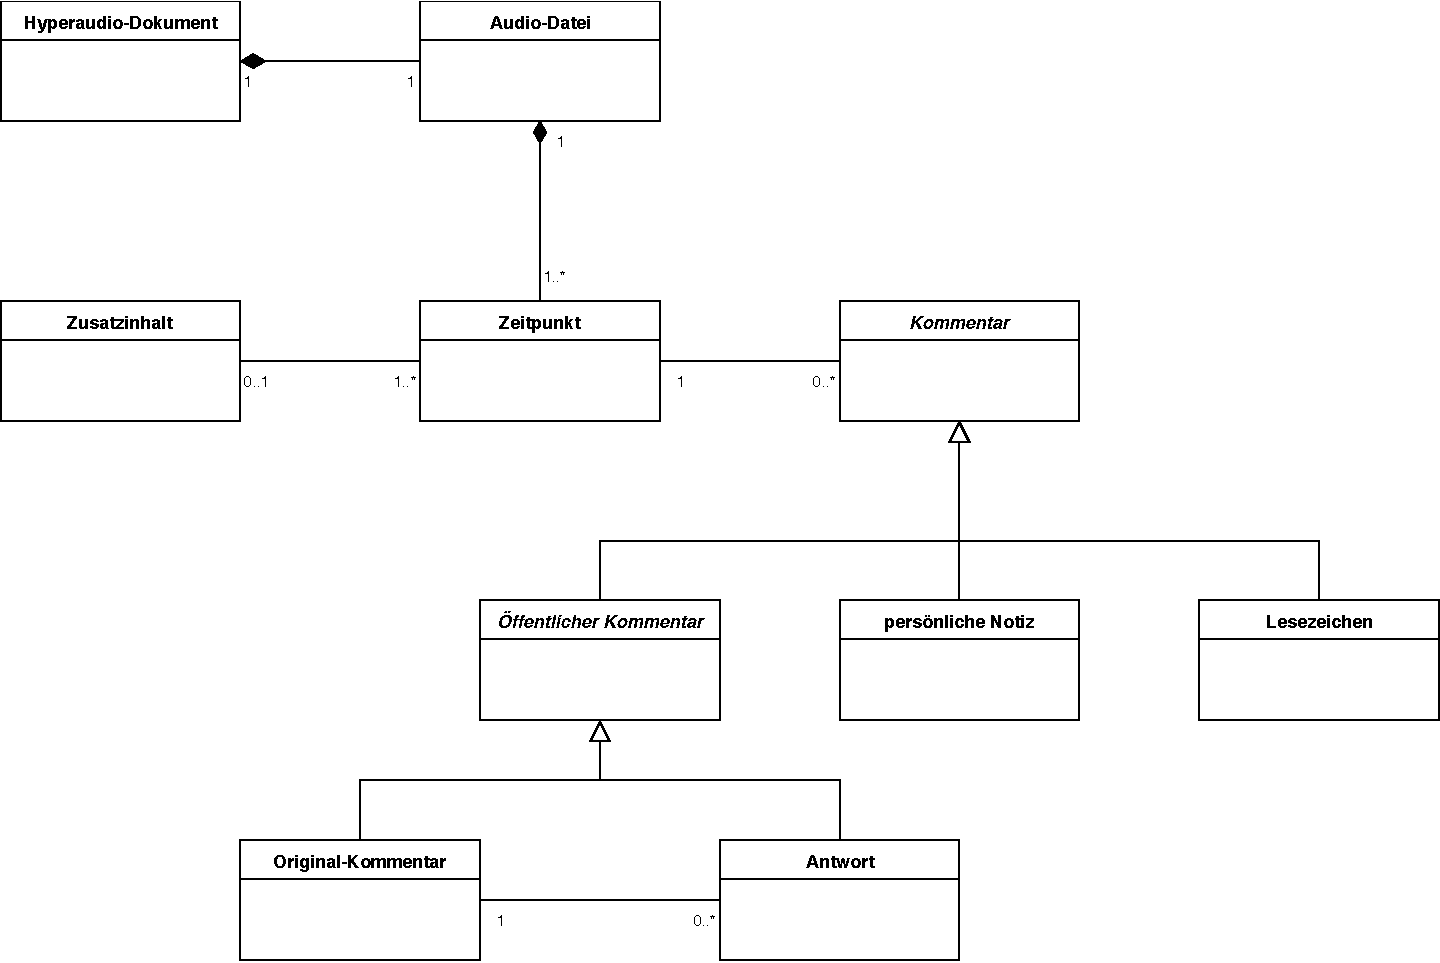
\includegraphics[width=\textwidth,center]{UMLZusammenhaenge.pdf}
\caption{\label{fig:UMLAufbau}Zusammenhänge der Komponenten}
\end{figure}


%%%%%%%%%%
\section{Definition des Schnittstellenformats für Hyperaudio"=Dokumente}
\label{sec:konfigurationsdatei}
Um ein Hyperaudio"=Dokument zu erstellen, können mehrere Dateien hochgeladen werden. Verpflichtend ist das Bereitstellen einer Audio-Datei sowie einer Konfigurationsdatei. Darin wird festgehalten, zu welchem Zeitpunkt welcher Zusatzinhalt annotiert werden soll. Darüber hinaus ist es mittels der Konfigurationsdatei möglich Metadaten (Name und Beschreibung des Zusatzinhalts sowie die betroffene Kurseinheit und die zugehörigen Seiten) für die einzelnen Zusatzinhalte und das Hyperaudio"=Dokument selbst anzufügen.
%Wie in der Einleitung dieses Kapitels beschrieben, kann die Konfiguration zu welchem Zeitpunkt welcher Zusatzinhalt annotiert werden soll mittels einer Konfigurationsdatei durchgeführt werden. Diese Vorgehensweise wird nun umgesetzt und die Konfigurationsdatei ist entsprechend zu definieren.
Aufgrund des Einsatzes von PHP und JavaScript innerhalb der Moodle-Plugin-Entwicklung bietet sich der Einsatz von JSON (JavaScript Object Notation) an. JSON wird direkt durch JavaScript unterstützt und bietet im Vergleich zu XML (Extensible Markup Language) erhebliche Geschwindigkeitsvorteile \citep{nurseitov2009comparison}.
%JSON is directly supported inside JavaScript [7] and is best suited for JavaScript applications; thus providing significant performance gains over XML, 
Mittels der JSON-Datei sollen die Informationen zum Autor des Hyperaudio"=Dokuments sowie folgende Informationen der Zusatzinhalte übertragen werden:

\begin{itemize}
\item Dateiname
\item Name des Zusatzinhaltes
\item Beschreibung des Zusatzinhaltes
\item Kurseinheit
\item Betroffene Seiten innerhalb der Kurseinheit
\item Startzeitpunkt der Annotation
\item Endzeitpunkt der Annotation
\end{itemize}

Entscheidend ist dabei vor allem der Dateiname. Anhand des Dateinamens kann anschließend die Zuordnung der weiteren Informationen zu der entsprechenden Audio-Datei in der Datenbank vorgenommen werden. Eine beispielhaft befüllte Konfigurationsdatei ist in Auflistung \ref{lst:JSON} dargestellt. 

\begin{lstlisting}[language=json,
             linewidth=\textwidth,
             caption={Beispielhafte Konfigurationsdatei},
             label={lst:JSON}]             
{
  "author": "Dr. Niels Seidel",
  "additional_contents": {
    "additional_content": [
      {"filename": "Abbildung_1_4.png",
      "name": "Abbildung 1.4",
      "course_unit": 1", 
      "page": "31",
      "description": "Ein kooperativer Editor zur Visualisierung von gemeinsam zu lernenden Vokabeln.",
      "begin": "5",
      "end": "10"},
      {"filename": "Abbildung_1_5.png",
      "name": "Abbildung 1.5",
      "course_unit": "1",
      "page": "32",
      "description": "Verschiedene Komponenten des Papierprototyps.",
      "begin": "62",
      "end": "220"}
    ]
  }
}
\end{lstlisting}

%%%%%%%%%%
\section{Datenbankentwurf}
\label{sec:datenbank}
Um die dem Plugin zugrundeliegende Datenbank zu gestalten, wird auf die Erkenntnisse aus Abschnitt \ref{sec:komponenten_zusammenhaenge} zurückgegriffen. Das Ergebnis ist dem ER-Diagramm in Abbildung \ref{fig:ERDiagramm} zu entnehmen.

Jede der Datenbanktabellen verfügt über einen Primärschlüssel (\textit{id}). Darüber hinaus wird zu jedem Eintrag gespeichert, wann dieser erstellt (\textit{timecreated}) und zuletzt bearbeitet (\textit{timemodified}) wurde. Für das Abspeichern von Dateien stellt Moodle die Tabelle \textit{files} bereit \citep{moodle2018file}. Dort kann die Datei abgelegt und an anderer Stelle darauf referenziert werden.

Im Mittelpunkt des Hyperaudio"=Plugins steht die Tabelle \textit{hyperaudio}. Diese repräsentiert das Hyperaudio"=Dokument als Ganzes und die Audio-Datei aus Abbildung \ref{fig:UMLAufbau}. Zunächst wird die ID des Moodle-Kurses (\textit{course}) abgelegt, dem das Hyperaudio"=Dokument zugeordnet ist. Während die Audio-Datei selbst in der bereits erwähnten Tabelle \textit{files} zu finden ist, wird in der Tabelle \textit{hyperaudio} deren Dateiname (\textit{audiofile}) festgehalten. Zum Hyperaudio"=Dokument können außerdem Name und Ersteller in den Spalten \textit{name} und \textit{author} hinterlegt werden. Eine optionale Beschreibung kann entsprechend dem de-facto-Standard der Moodle-Plugin-Entwicklung über \textit{introformat} und \textit{intro} hinzugefügt werden \citep{moodle2016activity}.

Bei der Tabelle \textit{hyperaudio\underline{{ }}config} handelt es sich um eine Tabelle, in welcher die in Abschnitt \ref{sec:konfigurationsdatei} beschriebene Konfigurationsdatei gespeichert wird (\textit{file} enthält den Dateinamen als Referenz auf die \textit{files}-Tabelle). Daneben wird nur noch der Fremdschlüssel \textit{hyperaudio\underline{{ }}id} auf die Tabelle \textit{hyperaudio} als Zuordnung zum Hyperaudio"=Dokument benötigt.

Zur Ablage der annotierten Zusatzinhalte dient die Tabelle \textit{additional\underline{{ }}content}. Auch hier steht der Name der Datei in der Spalte \textit{file} als Referenz auf die \textit{files}-Tabelle. Ebenso dient der Fremdschlüssel \textit{hyperaudio\underline{{ }}id} zur Verknüpfung des Zusatzinhalts mit der Audio-Datei. Des Weiteren werden folgende Metainformationen zum Zusatzinhalt abgespeichert:

\begin{itemize}

\item Name des Zusatzinhalts (\textit{name})
\item optional: Beschreibung (\textit{description})
\item optional: Kurseinheit (\textit{course\underline{{ }}unit})
\item optional: Seitenangabe (\textit{page})
\item Startzeitpunkt der Annotation innerhalb des Hyperaudio"=Dokuments (\textit{begin})
\item Endzeitpunkt der Annotation innerhalb des Hyperaudio"=Dokuments (\textit{end})

\end{itemize}

Die Tabelle \textit{hyperaudio\underline{{ }}comments} dient der Speicherung der vier in Abbildung \ref{fig:UMLAufbau} modellierten Kommentararten. Der Zusammenhang zum Hyperaudio"=Dokument wird analog per Fremdschlüssel \textit{hyperaudio\underline{{ }}id} hergestellt. Neben dem textuellen Kommentar (\textit{commenttext}), werden auch der Verfasser in Form der \textit{userid}, die Art des Kommentars (\textit{comment\underline{{ }}type})\footnote{\texttt{COMMENT}, \texttt{NOTE} oder \texttt{BOOKMARK}} und der Annotationszeitpunkt (\textit{timeannotated}) gespeichert. Für den Fall, dass es sich um einen Antwortkommentar handelt, wird in der Spalte \textit{comment\underline{{ }}id} die Referenz auf den Original-Kommentar festgehalten.

\begin{figure}[h!]
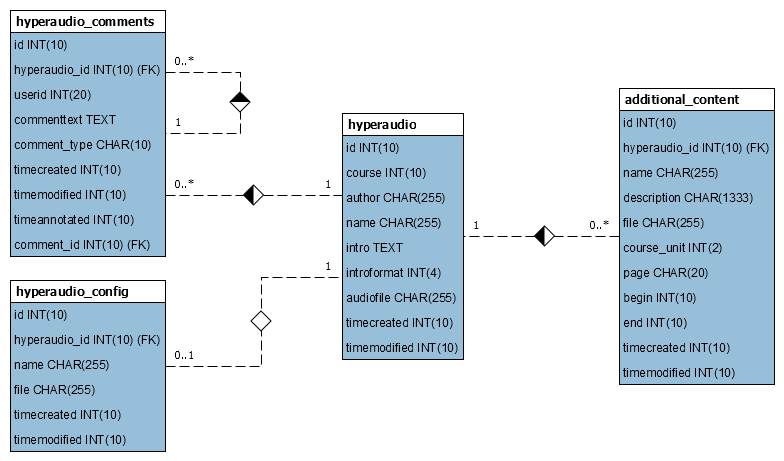
\includegraphics[width=\textwidth,center]{ERDiagramm.png}
\caption{\label{fig:ERDiagramm}ER-Diagramm der Datenbank des Moodle-Plugins}
\end{figure}


%%%%%%%%%%
\section{Gestaltung der Benutzeroberfläche}
Damit den Lehrenden und Studierenden die im vorherigen Kapitel beschriebenen Nutzungsszenarien möglichst leicht fallen, wird sich nun der Gestaltung der Benutzeroberfläche zugewandt. \glqq Das Design der Benutzeroberfläche stellt einen zentralen Aspekt für die Gebrauchstauglichkeit eines Softwareprodukts dar\grqq{} \citep[S. 1]{oppermann2002user}. Ein entsprechend hoher Stellenwert soll der Benutzeroberfläche des Hyperaudio"=Plugins zugeschrieben werden. Bei der Gestaltung der Benutzeroberfäche für die Darstellung der Hyperaudio-Aktivität wird die Ansicht in vier Bereiche aufgeteilt, welche in Abbildung \ref{fig:MockupBereiche} dargestellt sind.

\begin{figure}[h!]
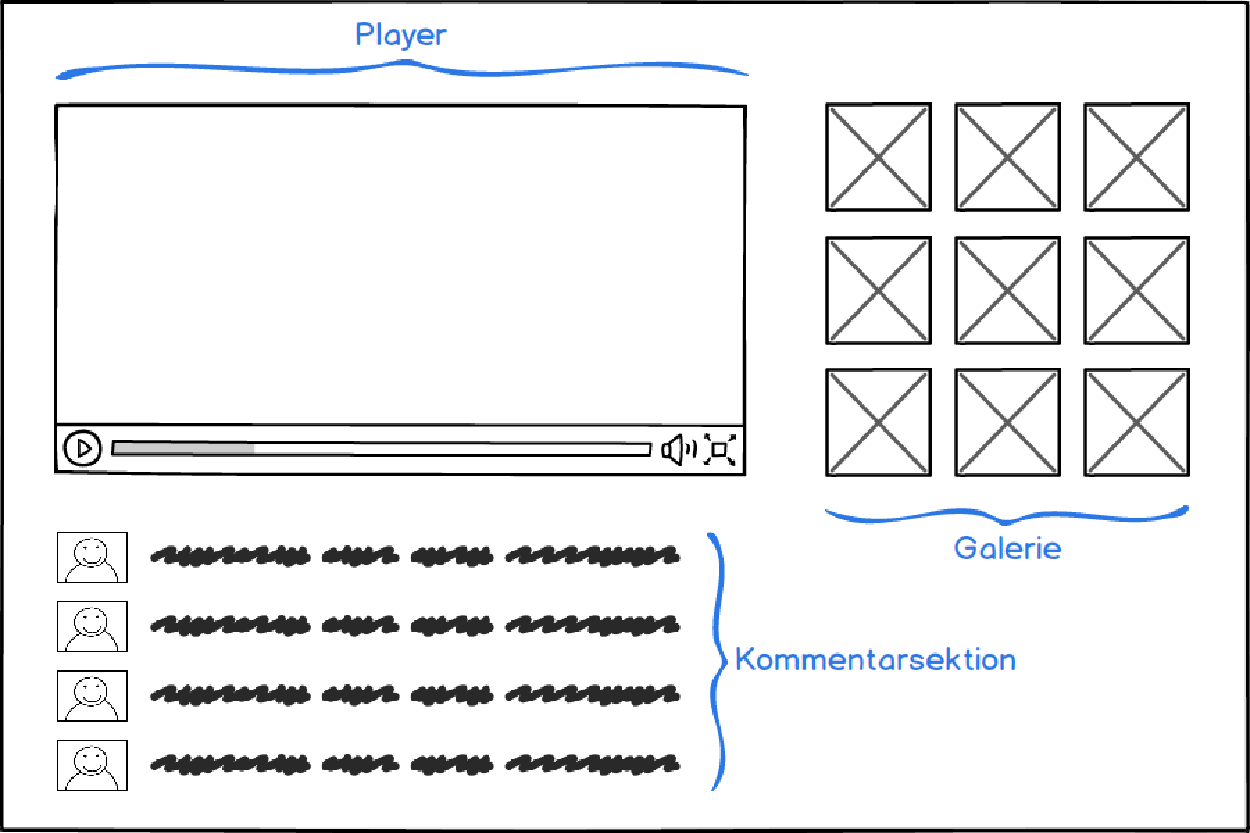
\includegraphics[width=0.8\textwidth,center]{MockupBereiche.pdf}
\caption{\label{fig:MockupBereiche} Bereiche einer Hyperaudio-Aktivität}
\end{figure}

Die Hyperaudio-Aktivität lässt sich demzufolge grob in die Bereiche \glqq Zusatzinhalte\grqq{}, \glqq Mediensteuerung inklusive Visualisierungen der Annotationen\grqq{}, \glqq Kommentare und Notizen\grqq{} und \glqq Galerie\grqq{} aufteilen. Zunächst werden nun für jeden dieser Bereiche verschiedene Designs erarbeitet und dann eines für die Verwendung im Hyperaudio"=Plugin festgelegt.

Generell erfolgen alle Entscheidungen bezüglich der Oberfläche auf Basis von Mockups. Diese wurden mithilfe des Programms \textit{Balsamiq Mockups 3.5.15}\footnote{https://balsamiq.com/} erstellt. Anhand der Skizzen können Vor- und Nachteile der verschiedenen Designansätze schnell erkannt und auf Grund dessen sachliche Entscheidungen getroffen werden. 

%%%%%%%%%%
\subsection{Zusatzinhalte}
\label{sub:zusatzinhalte}
Im Bereich der Zusatzinhalte beschränkt sich die Diskussion auf die Darstellung jener im vorhergesehen Bereich. So ist zu entscheiden, inwiefern die darzustellenden Zusatzinhalte auf die Größe des Bereichs skaliert werden sollen. Dabei ergeben sich folgende Möglichkeiten:

\begin{enumerate}
\item Beibehalten der originalen Größe
\item Anpassen auf die Größe des Bereichs ohne Berücksichtigung des Seitenverhältnisses
\item Anpassen auf die Größe des Bereichs unter Berücksichtigung des Seitenverhältnisses
\end{enumerate}

Die verschiedenen Möglichkeiten illustriert Abbildung\ref{fig:Zusatzinhalt}. Die erste Variante ist unpraktisch, da dies bei Inhalten, welche größer sind als der Bereich, dazu führt, dass nur ein Ausschnitt des Inhaltes dargestellt wird. Bei Inhalten, welche kleiner sind als der Bereich, wird hingegen nicht der volle Platz ausgenutzt und der Inhalt wird unnötig klein dargestellt. Bei der Variante 2 wird zwar stets der gesamte Bereich ausgenutzt und der Zusatzinhalt wird vollständig dargestellt, doch kann dies dazu zu unschönen Verzerrungen des dargestellten Inhaltes führen. Im Vergleich dazu bietet die dritte Variante den Vorteil, dass diese den Bereich möglichst gut ausnutzt ohne unschöne Verzerrungen zu verursachen.

\begin{figure}[h!]
\begin{subfigure}[c]{0.33\textwidth}
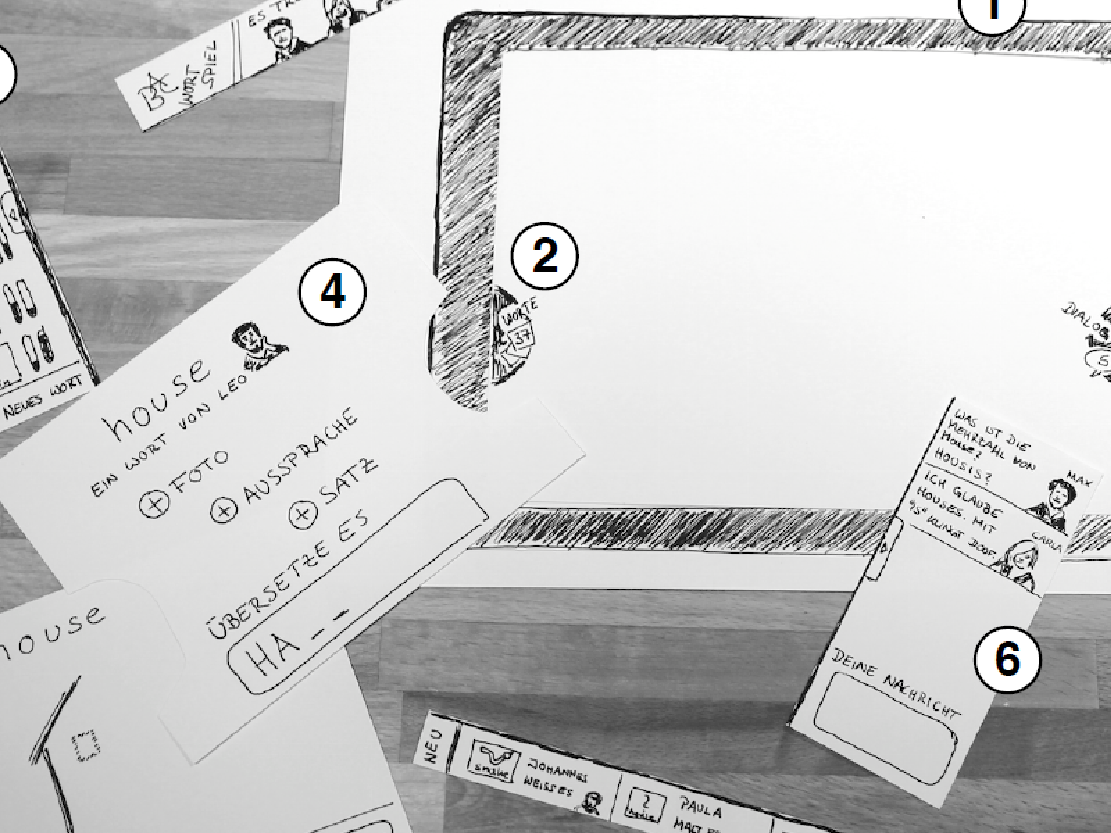
\includegraphics[width=0.9\textwidth,center]{Zusatzinhalt1.pdf}
\subcaption{Variante 1}
\label{fig:Zusatzinhalt1}
\end{subfigure}
\begin{subfigure}[c]{0.33\textwidth}
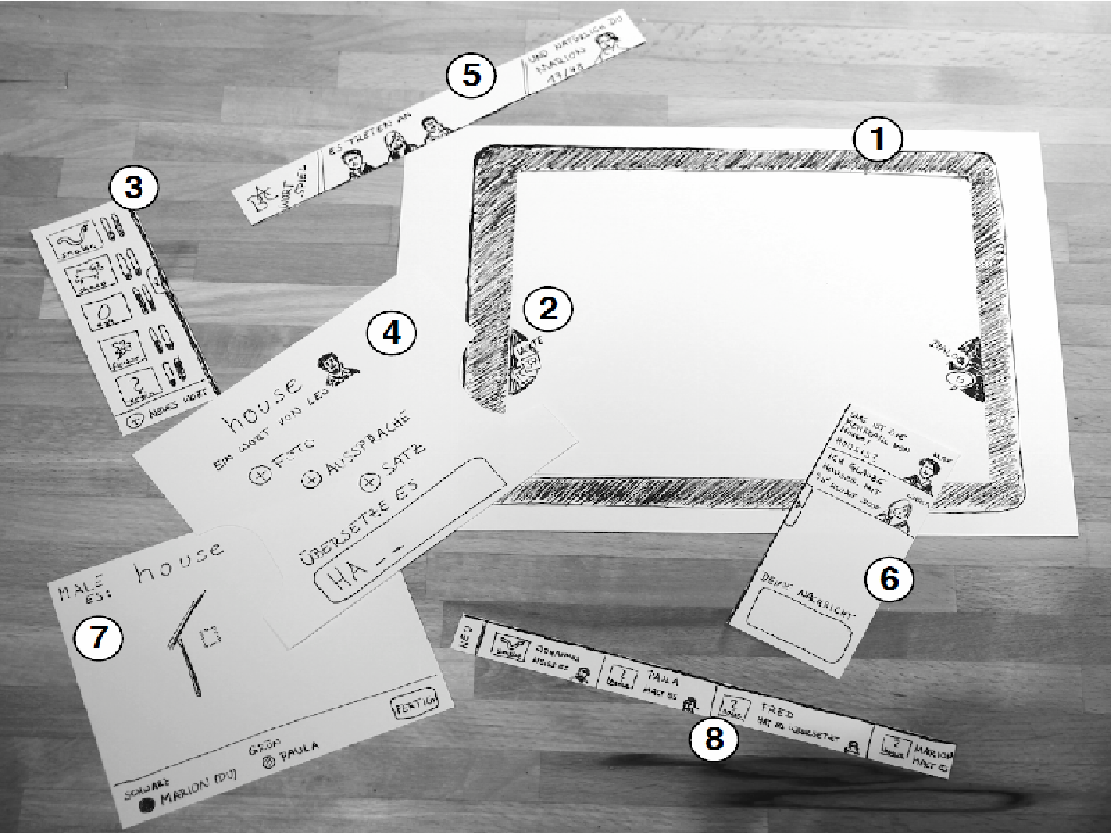
\includegraphics[width=0.9\textwidth,center]{Zusatzinhalt2.pdf}
\subcaption{Variante 2}
\label{fig:Zusatzinhalt2}
\end{subfigure}
\begin{subfigure}[c]{0.33\textwidth}
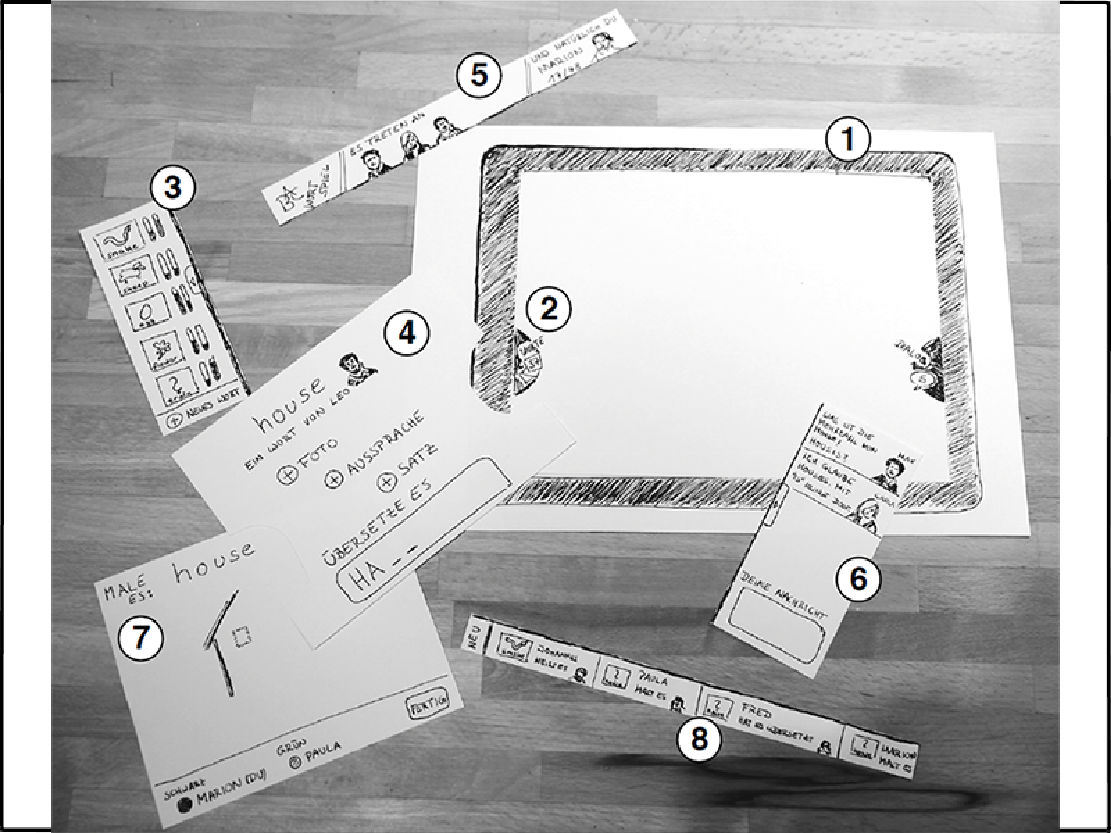
\includegraphics[width=0.9\textwidth,center]{Zusatzinhalt3.pdf}
\subcaption{Variante 3}
\label{fig:Zusatzinhalt3}
\end{subfigure}
\caption{Verschiedene Möglichkeiten zur Darstellung von Zusatzinhalten}
\label{fig:Zusatzinhalt}
\end{figure}

Neben der Entscheidung für Variante 3 muss auch die Entscheidung getroffen werden, wie sich der Bereich verhält, wenn gerade keine Zusatzinhalte dargestellt werden müssen. In diesem Fall sind verschiedene Szenarien denkbar. Zum einen wäre denkbar, dass der Bereich minimiert wird, sobald kein Zusatzinhalt dargestellt wird. Dies hätte aber den Nachteil, dass sich die Position der Kommentare mehrmals ändert und somit das Lesen erschwert wird. Zum anderen wäre auch die Darstellung eines Standardbildes oder einer einfarbigen Fläche vorstellbar. Es wäre aber auch möglich, innerhalb der Fläche die Metadaten des Hyperaudio"=Dokuments darzustellen, sprich Titel, Autor und Beschreibung. Die letzte Variante stellt einen guten Kompromiss dar, da somit auch keine weitere Fläche für die Darstellung dieser Informationen benötigt wird.

Darüber hinaus muss auch über das Darstellungsformat der Zusatzinhalte entschieden werden. Hierbei bieten sich die Formate 16:9 und 4:3 für die Darstellung an. Nachdem vornehmlich vorhandene Abbildungen, Formeln und Bilder aus bestehenden Kurseinheiten dargestellt werden sollen, fällt die Wahl auf das 4:3-Format, welches mehr Ähnlichkeiten mit dem DIN A4-Format von Kurseinheiten aufweist als das 16:9-Format. Letzteres würde sich eher für die Darstellung von Videos eignen.


%%%%%%%%%%
\subsection{Mediensteuerung inklusive Visualisierungen der Annotationen}
\label{sub:Mediensteuerung}
Bei der Mediensteuerung für Hyperaudio"=Dokumente sollen neben den üblichen Mediensteuerungselementen zusätzliche Informationen visualisiert werden. So sollen ähnlich wie bei \textit{SoundCloud} auch die annotierten öffentlichen Kommentare, persönlichen Notizen und Lesezeichen dargestellt werden. Die Möglichkeit zum Erstellen von Lesezeichen soll ebenfalls in die Mediensteuerung integriert werden. Anhand dieser erweiterten Mediensteuerung kann sich der Nutzende schnell einen Überblick über die Annotationen verschaffen.

Der erste Entwurf der Mediensteuerung ist in Abbildung \ref{fig:MockupMediensteuerungV1} dargestellt. Es ist zu erkennen, dass neben den üblichen Steuerungselementen die Visualisierung der Annotationen in der Timeline erfolgt. Hierzu wird für die drei verschiedenen Kommentar-Arten jeweils ein andersfarbiger Punkt (Kommentar: blau, Notiz: orange und Lesezeichen: grün) innerhalb der Timeline des Players dargestellt. Durch einen Klick auf einen Punkt, welcher einen Kommentar oder eine Notiz repräsentiert, soll dann zu der dazugehörigen Stelle innerhalb des Bereichs für Kommentare und Notizen gesprungen werden. Das Löschen und Anlegen von Lesezeichen soll durch eine Betätigung des Rechtsklicks auf den Punkt bzw. die Timeline möglich sein. Es wird ersichtlich, dass diese Variante den Nachteil hat, dass bei einer hohen Anzahl an Kommentaren und Notizen die Timeline unübersichtlich und schwer bedienbar wird.

In einem zweiten Entwurf der Mediensteuerung in Abbildung \ref{fig:MockupMediensteuerungV2} wird die Visualisierung der Notizen und Kommentare in eine Box unterhalb der Timeline verschoben. Diese werden nun in einer Waveform dargestellt. Hierfür wird jedes Hyperaudio"=Dokument in die gleiche fixe Anzahl an Zeitfenstern aufgeteilt. Diese Zeitfenster werden durch senkrecht orientierte Balken dargestellt, deren Höhe für die Anzahl der zu diesem Zeitfenster erfassten Kommentare und Notizen stehen soll. Die Balken werden anteilig nach Anzahl von Kommentaren und Notizen unterschiedlich eingefärbt. Dadurch wird nebenbei das Handling der Punkte in der Timeline vereinheitlicht, da es hier nur noch die Lesezeichen mit ihren Interaktionsmöglichkeiten gibt. Wenn mit der Maus über einen einzelnen Balken gefahren wird, soll jeweils eine Vorschau eines Kommentars mittels Tooltip dargestellt werden. Bei dem in der Vorschau angezeigten Kommentar handelt es sich um denjenigen Kommentar mit den meisten Antworten, also den meistdiskutierten Kommentar, innerhalb dieses Blockes. Wird hierbei kein eindeutiges Ergebnis gefunden, wird derjenige Kommentar mit dem frühesten Annotatioszeitpunkt herangezogen. Wenn weiterhin kein eindeutiges Ergebnis erzielt ist, wird der neueste dieser Kommentare in der Vorschau angezeigt. Bei einem Klick auf den Block wird zu der dazugehörigen Stelle innerhalb des Bereichs für Kommentare und Notizen gesprungen. Diese Version bietet somit auch bei einer hohen Anzahl an Kommentaren und Notizen eine übersichtliche Darstellung.

\begin{figure}[h!]
\begin{subfigure}[c]{\textwidth}
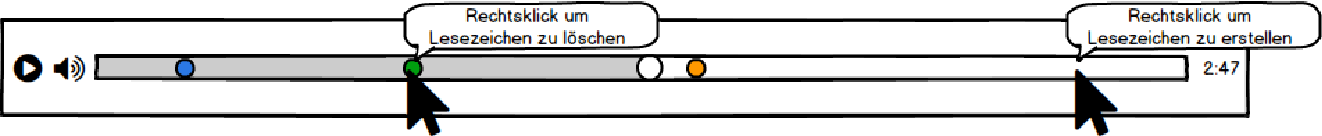
\includegraphics[width=0.8\textwidth,center]{MockupMediensteuerungV1.pdf}
\subcaption{Erste Version}
\label{fig:MockupMediensteuerungV1}
\end{subfigure}
\par\bigskip
\begin{subfigure}[c]{\textwidth}
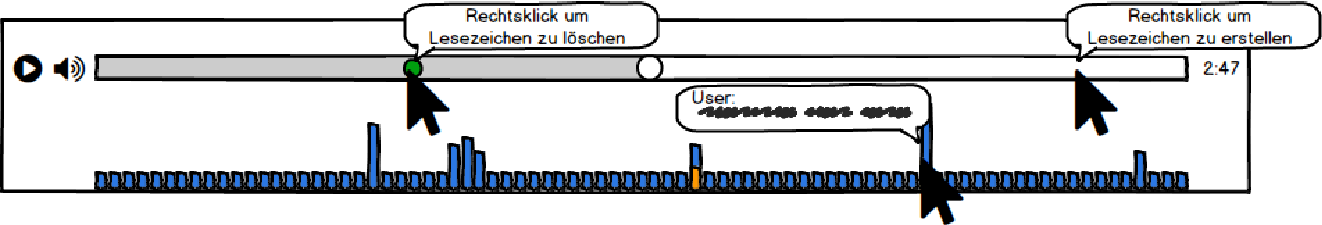
\includegraphics[width=0.8\textwidth,center]{MockupMediensteuerungV2.pdf}
\subcaption{Zweite Version}
\label{fig:MockupMediensteuerungV2}
\end{subfigure}
\par\bigskip
\begin{subfigure}[c]{\textwidth}
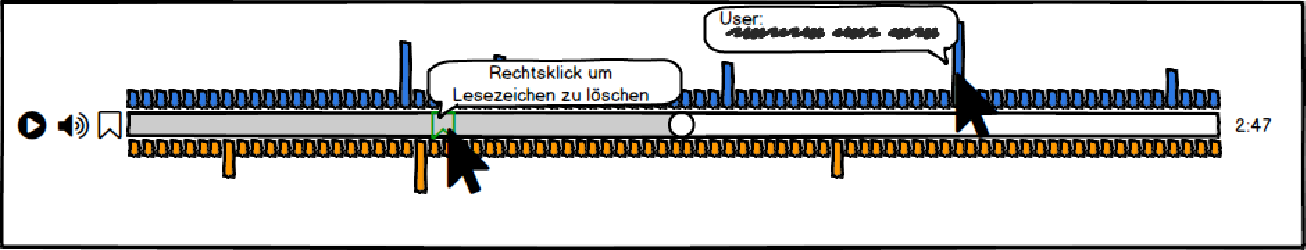
\includegraphics[width=0.8\textwidth,center]{MockupMediensteuerungV3.pdf}
\subcaption{Finale Version}
\label{fig:MockupMediensteuerungV3}
\end{subfigure}
\caption{Benutzeroberfläche - Mediensteuerung}
\label{fig:MockupMediensteuerung}
\end{figure}

In der dritten und finalen Variante wird die Waveform an die Timeline gedockt und zweigeteilt (siehe Abbildung \ref{fig:MockupMediensteuerungV3}). Der obere Teil repräsentiert die Kommentare, während der untere Teil die Notizen wiederspiegelt. Des Weiteren wurde ein Button zum Erstellen der Lesezeichen in der Mediensteuerung ergänzt. Somit ist nur noch zum Löschen der Lesezeichen die Verwendung des Rechtsklicks notwendig. Darüber hinaus wurde der Punkt für Lesezeichen durch ein dediziertes Symbol ersetzt. Diese Version bietet den Vorteil, dass die Interaktion, welche in der vorherigen Version ausschließlich Kommentaren vorbehalten war, ebenfalls für Notizen eingebettet werden kann. Demnach ist es auch möglich, in der Mediensteuerung mittels Mouseover eine Vorschau einer Notiz anzeigen zu lassen und mit Klick zu dieser zu springen. Durch die neue Art der Visualisierung von Kommentaren, Notizen und Lesezeichen wird zudem die Barrierefreiheit der Anwendung verbessert, da die Kommentararten nicht nur anhand der Farbe zu unterscheiden sind, sondern auch anhand der Positionierung.

%%%%%%%%%%
\subsection{Galerie}
Die Galerie soll dazu dienen, einen Überblick über die vorhanden Zusatzinhalte zu bieten. Da die Zusatzinhalte alle einen grafischen Inhalt darstellen, kann jeder Zusatzinhalt durch ein kleines Vorschaubild repräsentiert werden. Hier wird in Fragen der Skalierung die gleiche Entscheidung getroffen wie bereits bei der Darstellung von Zusatzinhalten (vgl. Abschnitt \ref{sub:zusatzinhalte}).
Eine weitere Grundfunktionalität einer Galerie ist die vergrößerte Anzeige der in der Vorschau dargestellten Inhalte, die auch in der Hyperaudio-Galerie zur Verfügung stehen soll. Um den Komfort zu erhöhen und den Hyperaudio-Gedanken zu stärken, ist eine Rückkopplung an die Mediensteuerung vorgesehen.

Die simpelste Umsetzung der Galerie ist eine Darstellung der Zusatzinhalte in einem einfachen Grid  mit Scrollbalken, wie es in Abbildung \ref{fig:MockupGalerieGrid} zu sehen ist. Zusätzlich wird das Grid um zwei Buttons für eine vergrößerte Ansicht des Zusatzinhalts sowie für die Rückkopplung zur Mediensteuerung ergänzt. Um eine dieser beiden Aktionen auszuführen, müsste also der gewünschte Zusatzinhalt markiert und der entsprechende Button betätigt werden.

Diese Variante hat den Vorteil, dass besonders viele Zusatzinhalte gleichzeitig angezeigt werden können. Auf der anderen Seite wird aber keinerlei Informationen zu den Zusatzinhalten geliefert. In der zweiten Variante, bei dem das Grid um einen Bereich für Details ergänzt wurde, kann der Nutzer zumindest die Details des ausgewählten Zusatzinhaltes einsehen. Diese in Abbildung \ref{fig:MockupGalerieGridErweitert} erkennbaren Details sind natürlich von den vorhandenen Metadaten abhängig. Nachteil ist in diesem Fall aber, dass durch den zusätzlichen Bereich für die Details bei gleicher Größe der Galerie weniger Zusatzinhalte zur selben Zeit dargestellt werden können. Das führt dazu, dass die Verwendung des Scrollbalkens häufiger notwendig wird.

Bei einer Darstellung der Zusatzinhalte als Kacheln, wie in Abbildung \ref{fig:MockupGalerieKacheln} zu sehen, können gleichzeitig für alle vorhandenen Zusatzinhalte Details angezeigt werden. Durch diese Art der Darstellung passen jedoch noch weniger Zusatzinhalte auf die gleiche Fläche.

Eine besonders elegante Art der Darstellung wäre die des Cover Flows, bekannt aus verschiedenen Musikplayern, wie beispielsweise \textit{iTunes}. In Abbildung \ref{fig:MockupGalerieCoverFlow} ist zu erkennen, dass auch hier ausschließlich Details des aktuell ausgewählten Zusatzinhaltes sichtbar sind. Des Weiteren hat diese Darstellungsweise den großen Nachteil, dass nicht auf einen Blick alle verfügbaren Zusatzinhalte ersichtlich sind, was das Durchsuchen der Zusatzinhalte ungemein erschwert. Somit ist diese Art der Darstellung zwar schön anzusehen, aber nicht sonderlich gebrauchstauglich im Zusammenhang mit Hyperaudio"=Dokumenten.

Letztlich stellt sich die optimierte Variante der Kachel-Darstellung in Abbildung \ref{fig:MockupGalerieFinal} als beste Lösung heraus. Die Optimierung besteht darin, dass die beiden Buttons obsolet gemacht werden. Dies kann zum einen dadurch erreicht werden, dass die vergrößerte Darstellung durch einen Klick auf das Vorschaubild ausgelöst wird. Zum anderen bietet der Bereich der Details noch ausreichend Platz, um hier die Funktion zur Rückkopplung an die Mediensteuerung einzufügen. Durch diese Verbesserungen wird nicht nur mehr Platz geschaffen, sondern auch die Benutzerfreundlichkeit erhöht, da der Vorgang zum Anzeigen der vergrößerten Ansicht beziehungsweise des Springens an den entsprechenden Zeitpunkt jeweils um einen Klick reduziert wurde.

\begin{figure}[h!]
\begin{subfigure}[c]{0.5\textwidth}
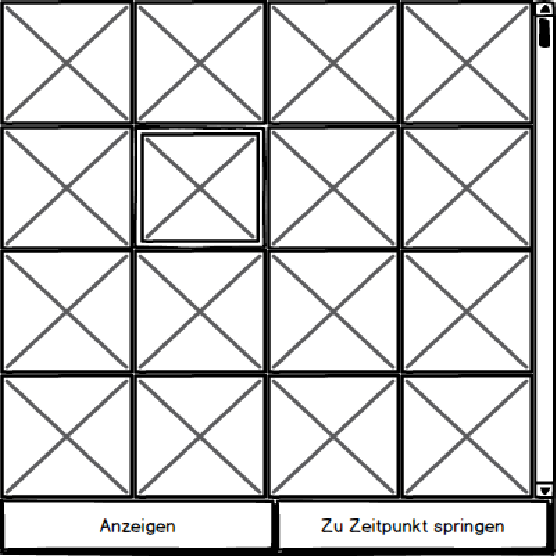
\includegraphics[width=0.8\textwidth,center]{MockupGalerieGrid.pdf}
\subcaption{Galerie als einfaches Grid}
\label{fig:MockupGalerieGrid}
\end{subfigure}%
\begin{subfigure}[c]{0.5\textwidth}
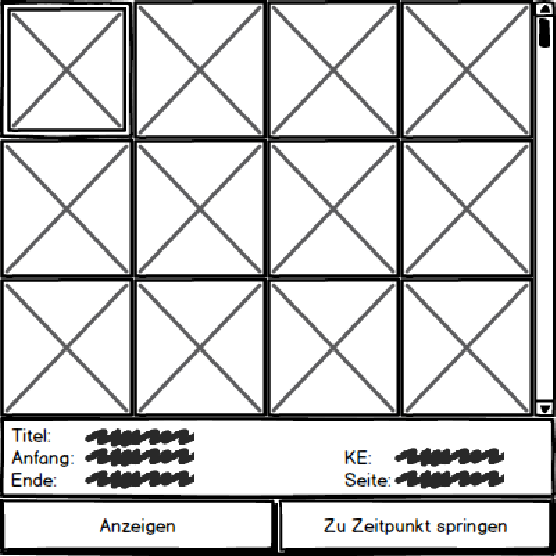
\includegraphics[width=0.8\textwidth,center]{MockupGalerieGridErweitert.pdf}
\subcaption{Galerie als Grid mit Bereich für Details}
\label{fig:MockupGalerieGridErweitert}
\end{subfigure}
\par\bigskip
\begin{subfigure}[c]{0.5\textwidth}
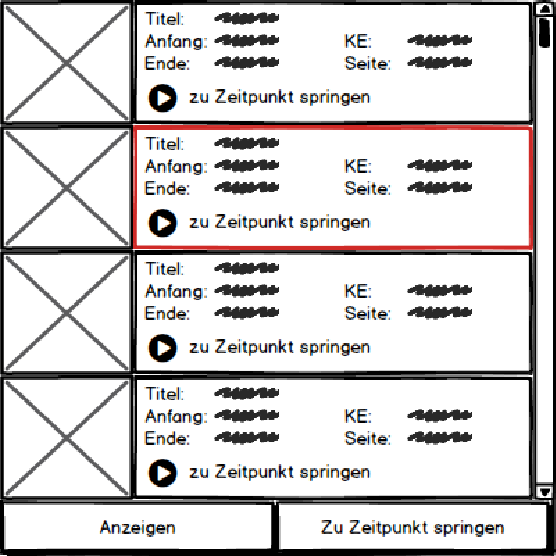
\includegraphics[width=0.8\textwidth,center]{MockupGalerieKacheln.pdf}
\subcaption{Galerie mit Darstellung in Kachelform}
\label{fig:MockupGalerieKacheln}
\end{subfigure}%
\begin{subfigure}[c]{0.5\textwidth}
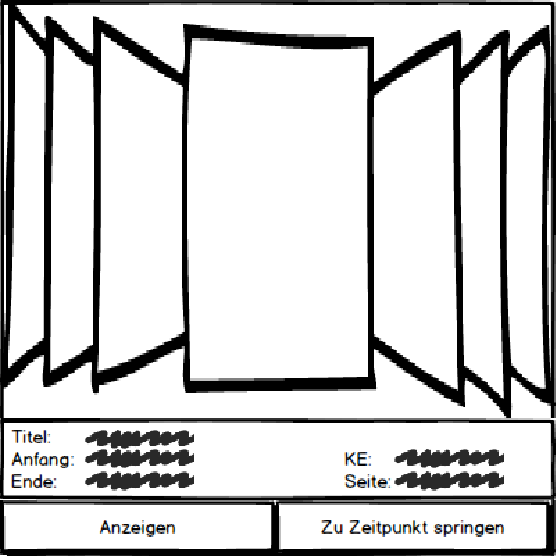
\includegraphics[width=0.8\textwidth,center]{MockupGalerieCoverFlow.pdf}
\subcaption{Galerie als Cover Flow}
\label{fig:MockupGalerieCoverFlow}
\end{subfigure}
\par\bigskip
\begin{subfigure}[c]{\textwidth}
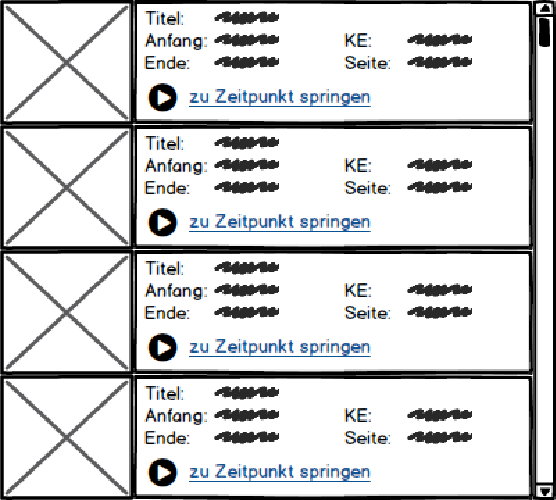
\includegraphics[width=0.4\textwidth,center]{MockupGalerieFinal.pdf}
\subcaption{Finale Version der Galerie}
\label{fig:MockupGalerieFinal}
\end{subfigure}
\caption{Benutzeroberfläche - Galerie}
\label{fig:MockupGalerie}
\end{figure}

%%%%%%%%%%
\subsection{Kommentare und Notizen}
Der Kommentarbereich ist für das Erstellen und Anzeigen der öffentlichen Kommentare sowie der persönlichen Notizen zuständig. Zusätzlich müssen eine Suche, Filter- und Sortiermöglichkeiten auf Basis der Anforderungen aus Abschnitt \ref{sub:AnforderungenDerNutzenden} in die Oberfläche integriert werden.

\begin{figure}[h!]
\begin{subfigure}[c]{\textwidth}
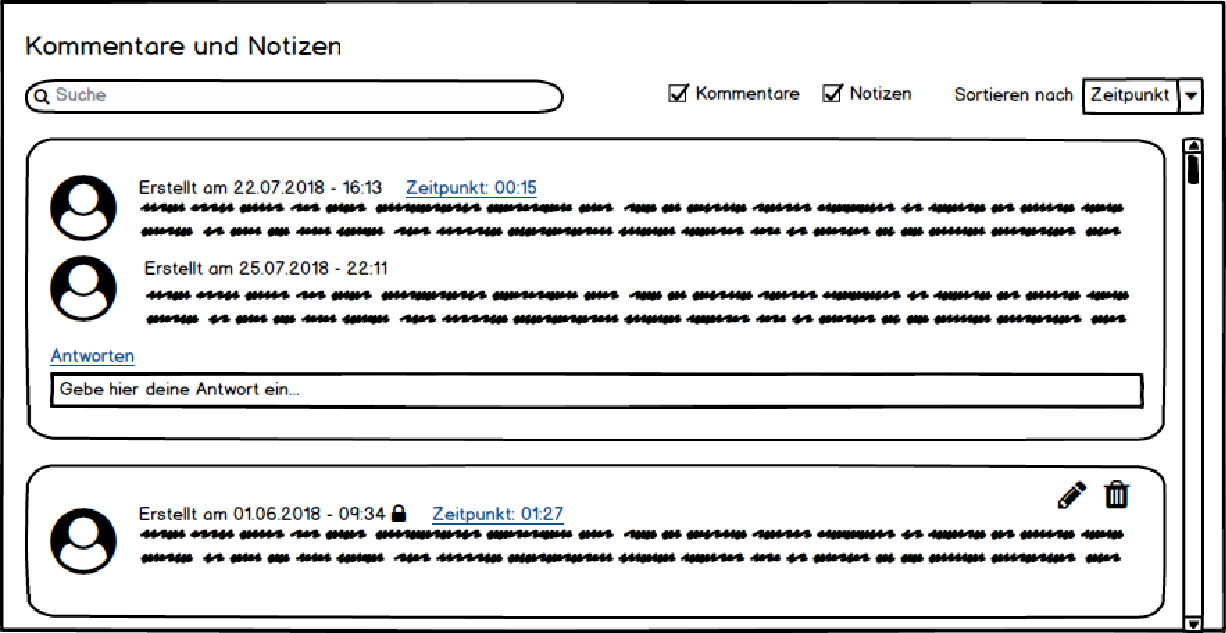
\includegraphics[width=\textwidth,center]{MockupKommentarsektionVersion1.pdf}
\subcaption{Erste Version}
\label{fig:MockupKommentarsektionVersion1}
\end{subfigure}
\par\bigskip
\begin{subfigure}[c]{\textwidth}
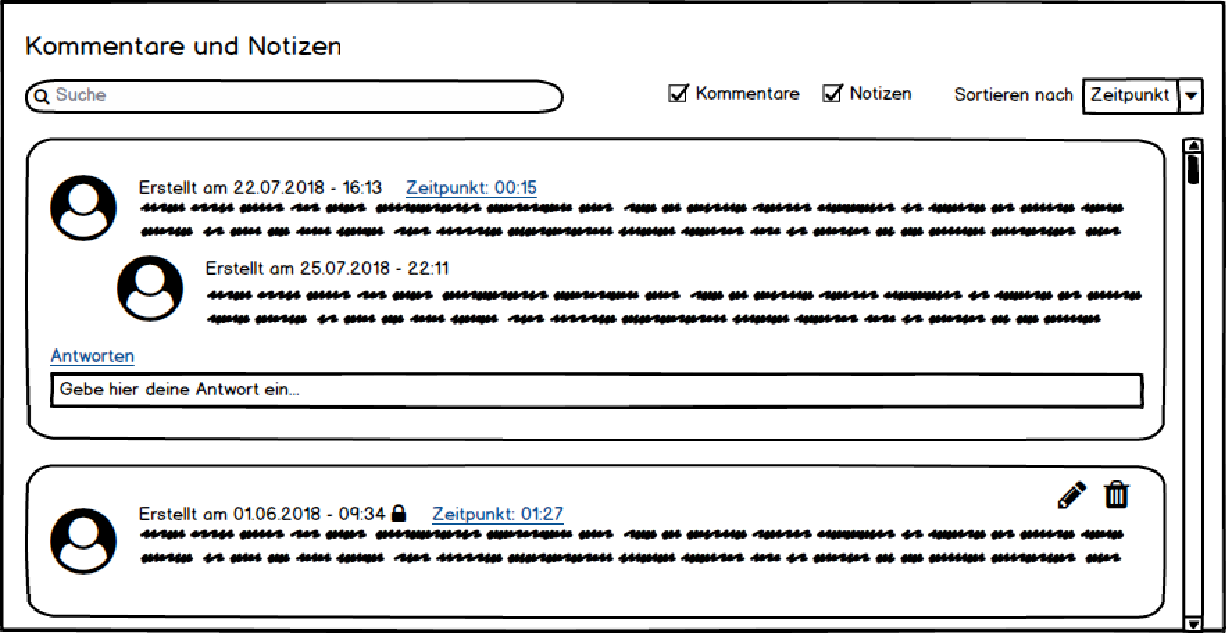
\includegraphics[width=\textwidth,center]{MockupKommentarsektionFinal.pdf}
\subcaption{Finale Version}
\label{fig:MockupKommentarsektionFinal}
\end{subfigure}
\caption{Benutzeroberfläche - Bereich für Kommentare und Notizen}
\label{fig:MockupKommentarsektion}
\end{figure}

\FloatBarrier

Abbildung \ref{fig:MockupKommentarsektionVersion1} zeigt eine erste Version des Kommentarbereichs. An oberste Stelle befinden sich eine Eingabemaske für Kommentare mit zwei Buttons, um den Inhalt der Eingabemaske als Kommentar oder Notiz abzuspeichern. Darunter befindet sich eine Suchmaske, neben dieser werden zwei Checkboxen dargestellt. Diese ermöglichen es dem Betrachter nach öffentlichen Kommentaren und persönlichen Notizen zu filtern. Im benachbarten Dropdown-Menü kann die Grundlage der Sortierung bestimmt werden. Die Sortierung kann nach Erstellungsdatum beziehungsweise nach Zeitpunkt der Annotation innerhalb des Hyperaudio"=Dokuments erfolgen.\\
Unterhalb dieser Funktionen befindet sich die Anzeige der Kommentare und Notizen. Sowohl bei Kommentaren als auch bei Notizen wird neben dem Erstellungsdatum auch der Annotationszeitpunkt festgehalten. Dieser wird als Link umgesetzt, sodass analog zur Galerie bei einem Klick die Rückkopplung an die Mediensteuerung erfolgen kann.\\
Bei Kommentaren gibt es nach Betätigung der \textit{Antworten}-Schaltfläche noch eine zusätzliche Eingabemaske zum Verfassen von Antworten. Damit die Kommunikation zwischen Studierenden und Lehrenden stets nachvollziehbar bleibt, werden weder eine Bearbeitungs- noch eine Löschfunktion für Kommentare und Antworten zur Verfügung gestellt.\\
Bei persönlichen Notizen hingegen wird das Bearbeiten und Löschen durch zwei zusätzliche Schaltflächen ermöglicht. Persönliche Notizen werden durch ein Schloss-Symbol hinter dem Erstellungsdatum gekennzeichnet.

Im nochmals verbesserten Design, welches in Abbildung \ref{fig:MockupKommentarsektionFinal} abgebildet ist, werden die Antworten auf Kommentare eingerückt dargestellt. Diese Darstellung führt zu einer verbesserten Übersicht und ist auch aus anderen modernen Anwendungen (wie zum Beispiel \textit{SoundCloud} und \textit{Youtube}, vgl. Abschnitt \ref{sec:Technik}) bekannt.

%%%%%%%%%%
\subsection{Zusammenführen der Elemente}
Im ersten Schritt werden die jeweils favorisierten Elemente in ein Layout zusammengeführt. Dabei wird sich zunächst an der groben Skizze aus Abbildung \ref{fig:MockupBereiche} orientiert. Wie nun in Abbildung \ref{fig:MockupSeiteLayoutVersion1} zu erkennen ist, wird der Anzeige der Zusatzinhalte und der Mediensteuerung eine große Fläche der Seite zugesprochen. Somit soll zugesichert werden, dass die Zusatzinhalte lesbar dargestellt werden. In dieser ersten Version ist der Bereich der Kommentare und Notizen so in die Breite gezogen, dass das Lesen der Inhalte auf großen Bildschirmen unangenehm werden kann. Aus diesem Grund wird in der finalen Version (siehe Abbildung \ref{fig:MockupSeiteLayoutFinal}) die Breite dieses Bereichs auf die Breite der Zusatzinhalte und Mediensteuerung beschränkt. Dies hat zeitgleich zur Folge, dass der nun vorhandene freie Platz für die Galerie verwendet werden kann. Spätestens hiermit wird der Nachteil der gewählten Darstellungsweise der Galerie egalisiert, da nun ausreichend viele Zusatzinhalte ohne die Verwendung des Scrollbalkens eingesehen werden können.

\begin{figure}[h!]
\begin{subfigure}[c]{\textwidth}
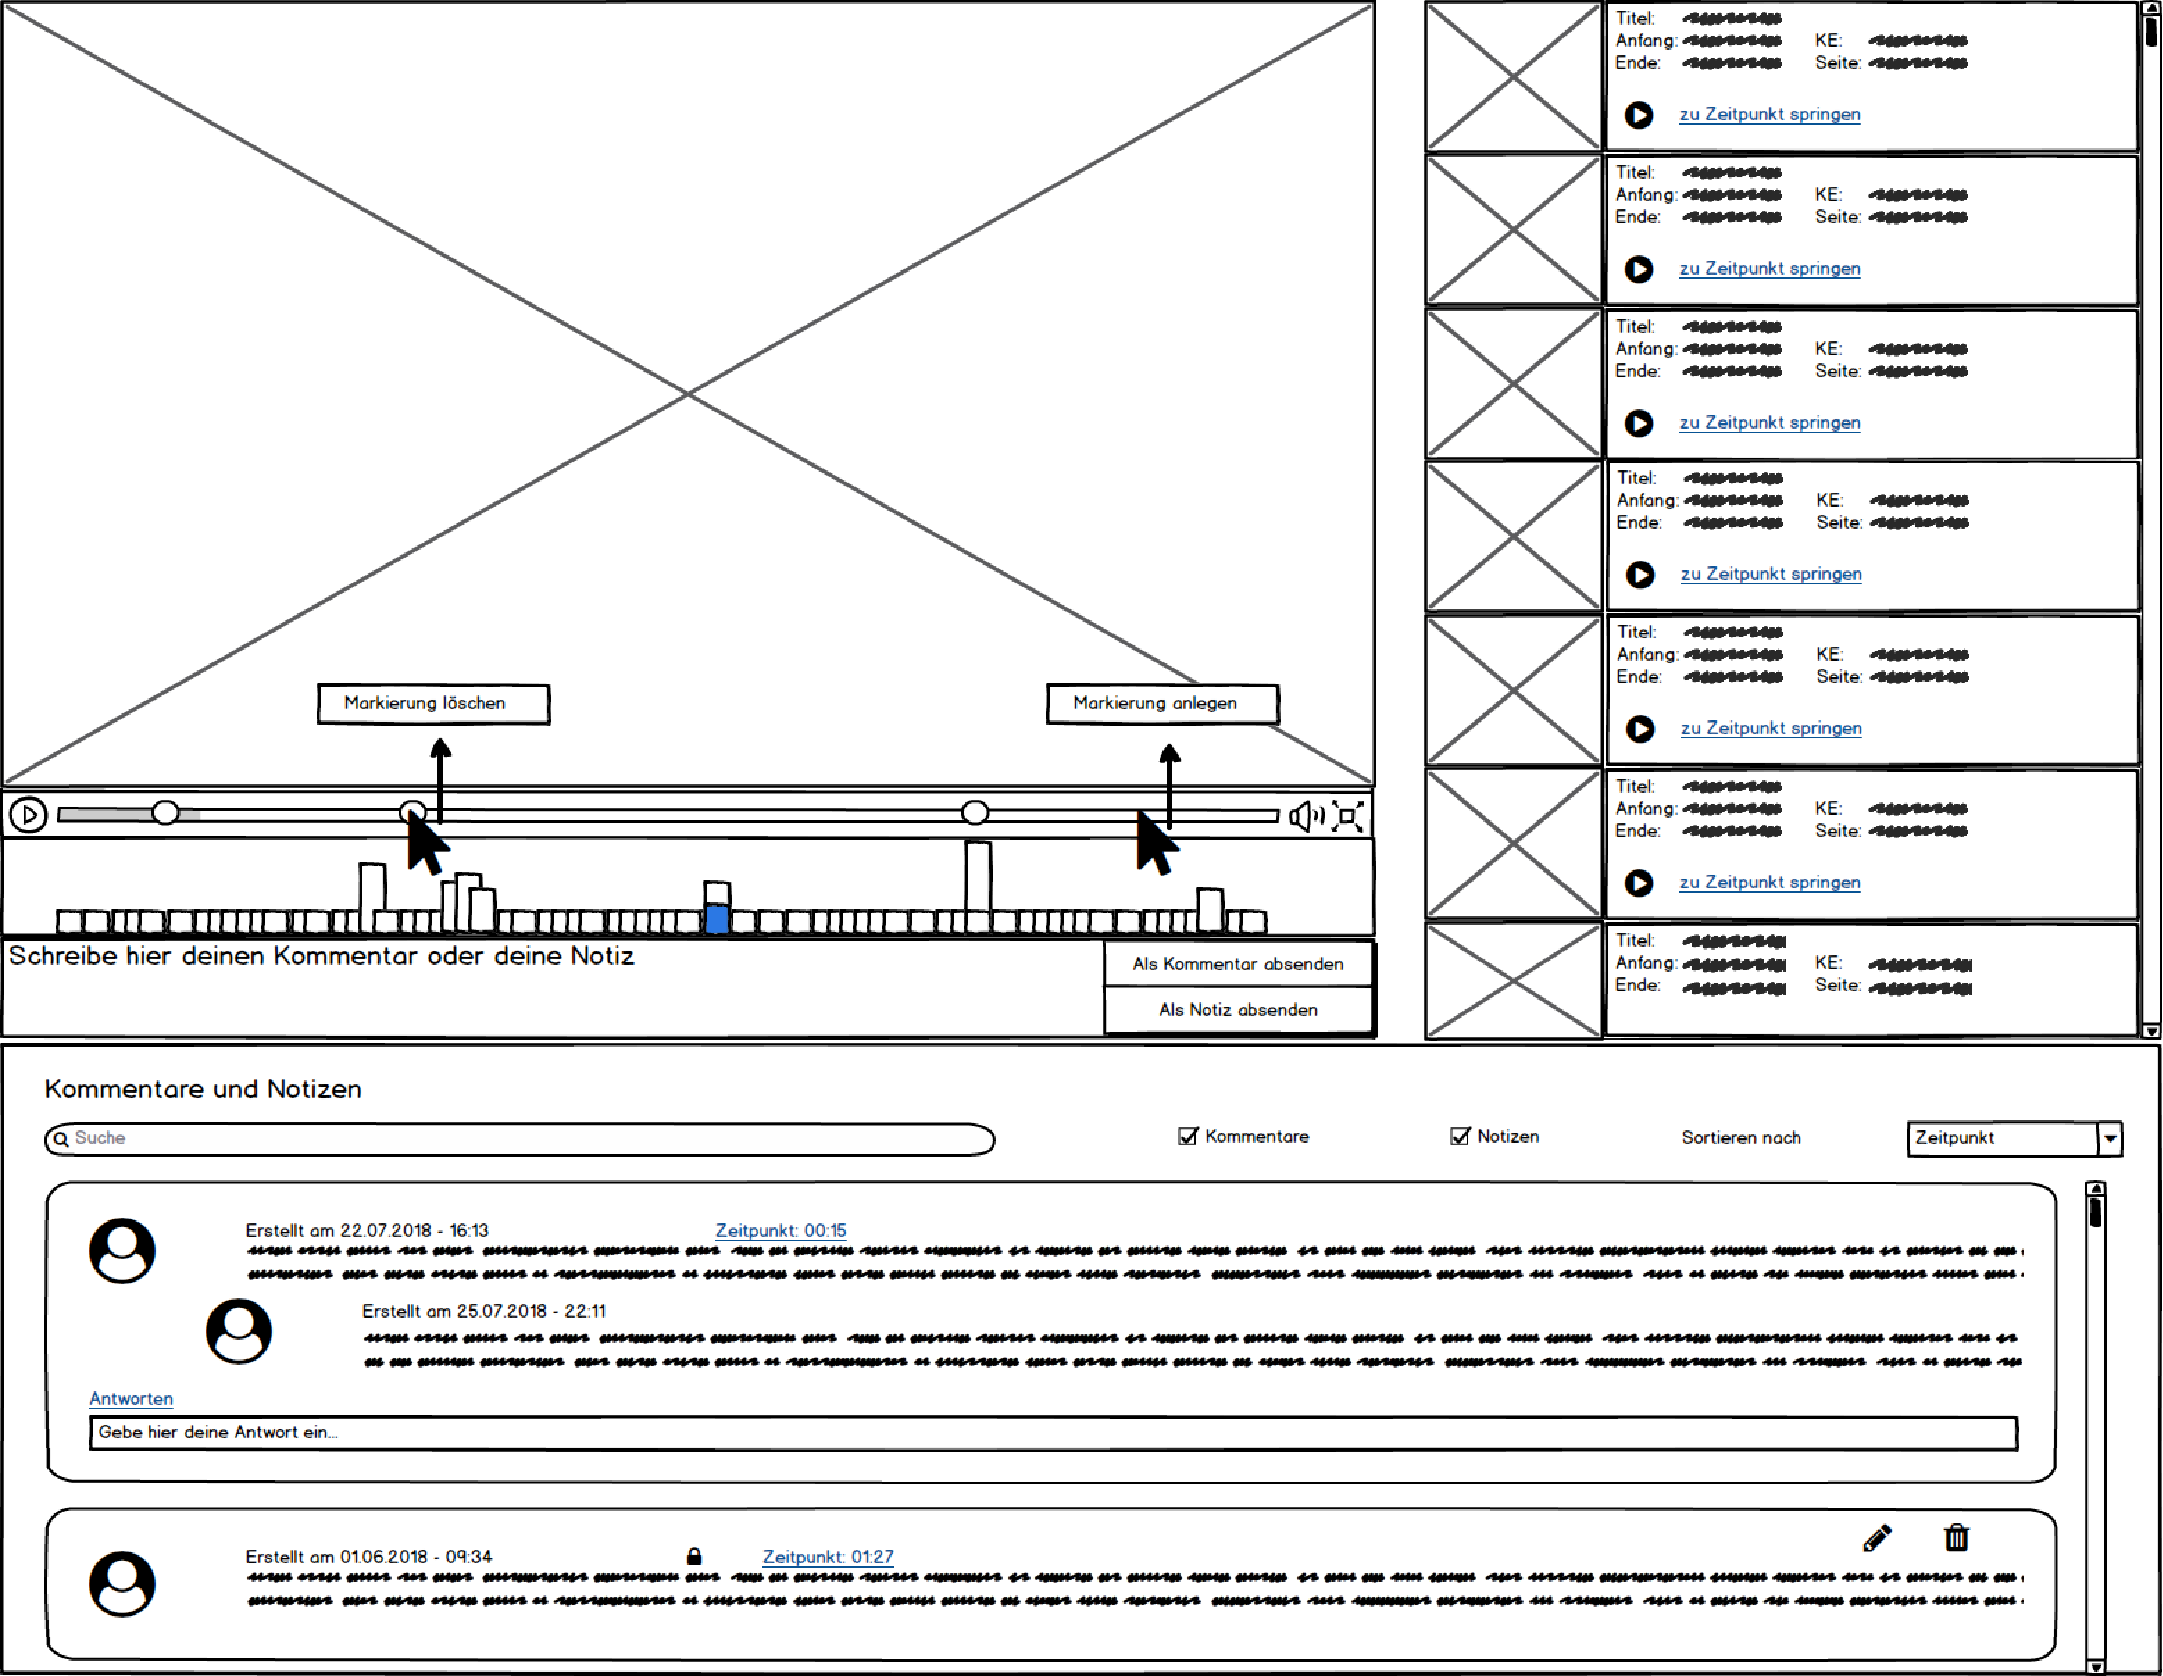
\includegraphics[width=0.67\textwidth,center]{MockupSeiteLayoutVersion1.pdf}
\subcaption{Erste Version}
\label{fig:MockupSeiteLayoutVersion1}
\end{subfigure}
\par\bigskip
\begin{subfigure}[c]{\textwidth}
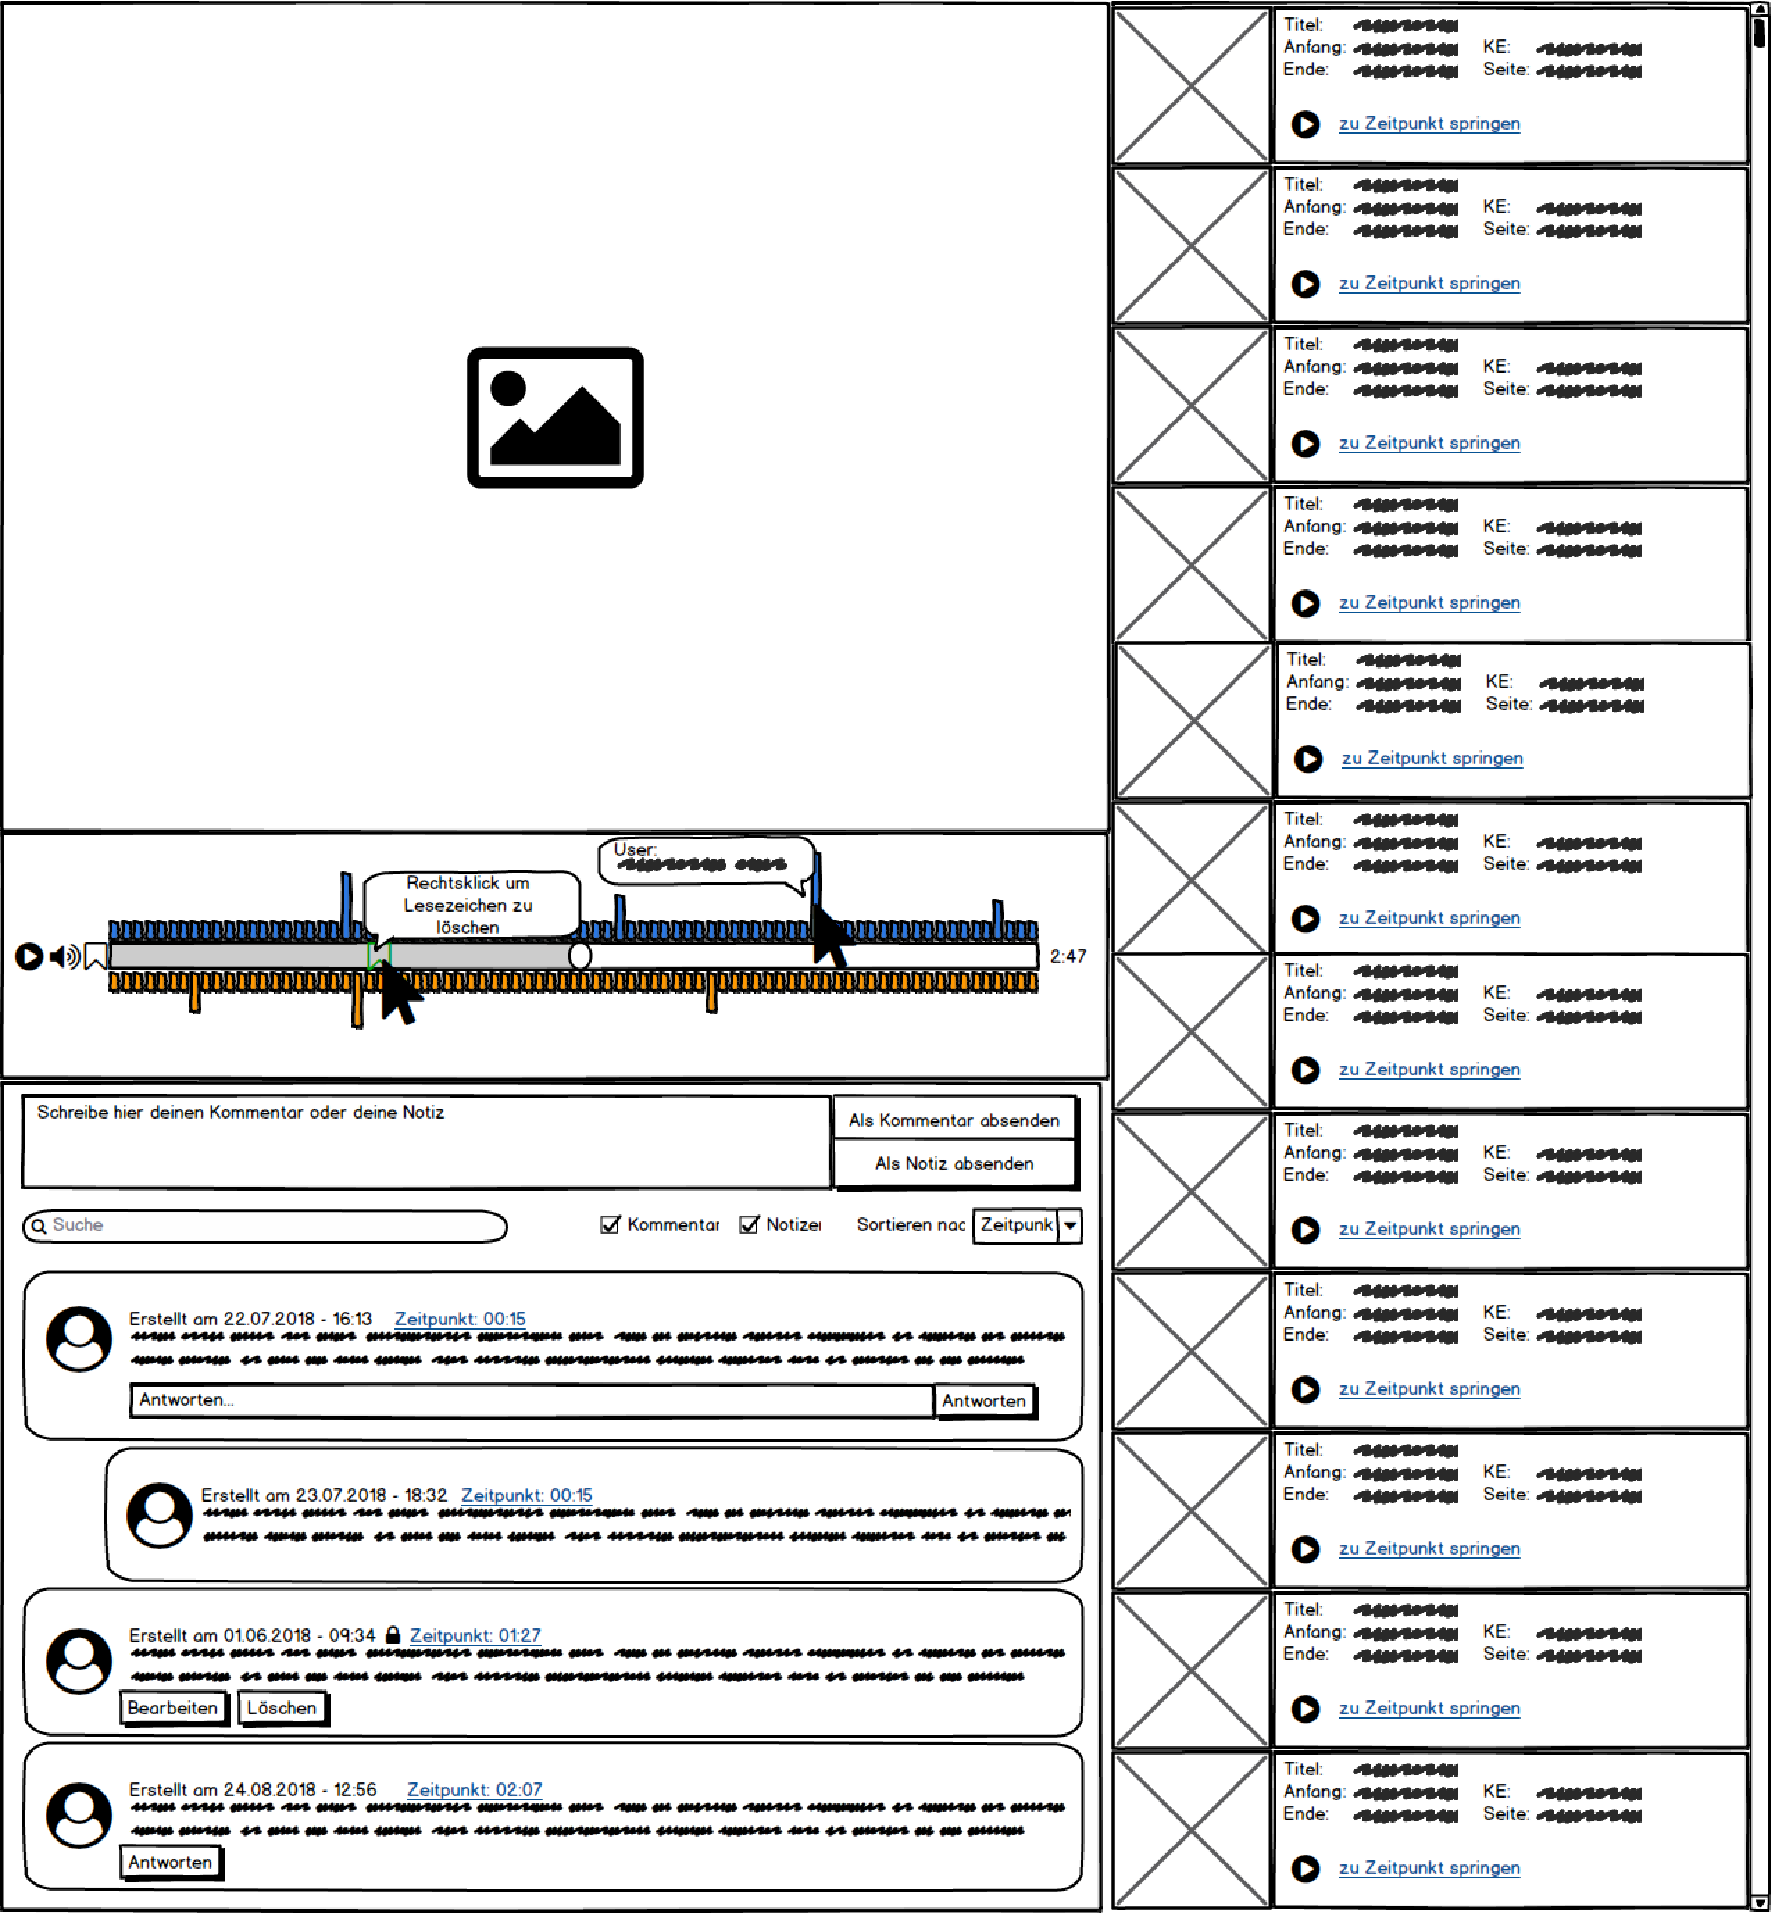
\includegraphics[width=0.67\textwidth,center]{MockupSeiteLayoutFinal.pdf}
\subcaption{Finale Version}
\label{fig:MockupSeiteLayoutFinal}
\end{subfigure}
\caption{Benutzeroberfläche - Zusammengeführtes Layout}
\label{fig:MockupSeiteLayout}
\end{figure}

%%%%%%%%%%
\subsection{Mobile Version}
\label{sub:mobile}
Für mobile Endgeräte wird keine neue Benutzeroberfläche entworfen. Stattdessen wird die vorhandene Oberfläche so angepasst (siehe Abbildung \ref{fig:MockupMobile}), dass diese für die Darstellung auf mobilen Geräten geeignet ist. Dazu wird die Strategie eines responsiven Grid-Layouts angewandt, das dafür sorgt, dass Inhalte bei kleineren Bildschirmgrößen anhand definierter Breakpoints umgebrochen werden \citep{hellichtresponsive}.

So wird beispielsweise die Galerie auf kleinen Displays unterhalb des Bereichs für Kommentare und Notizen platziert. Dasselbe Vorgehen erstreckt sich auf weitere Bedienelemente, wie zum Beispiel die Filtermöglichkeiten. Zudem wird die Anzahl der Balken zur Visualisierung von Annotationen im Bereich der Mediensteuerung abhängig von der zur Verfügung stehenden Bildschirmgröße gewählt, sodass diese jeweils gut erkennbar bleiben und dabei möglichst viel Information liefern. Die Mediensteuerung selbst sowie die Anzeige der Zusatzinhalte skaliert mit der Bildschirmbreite, jedoch nur bis zu einer definierten Maximalbreite.

\FloatBarrier

\begin{figure}[h!]
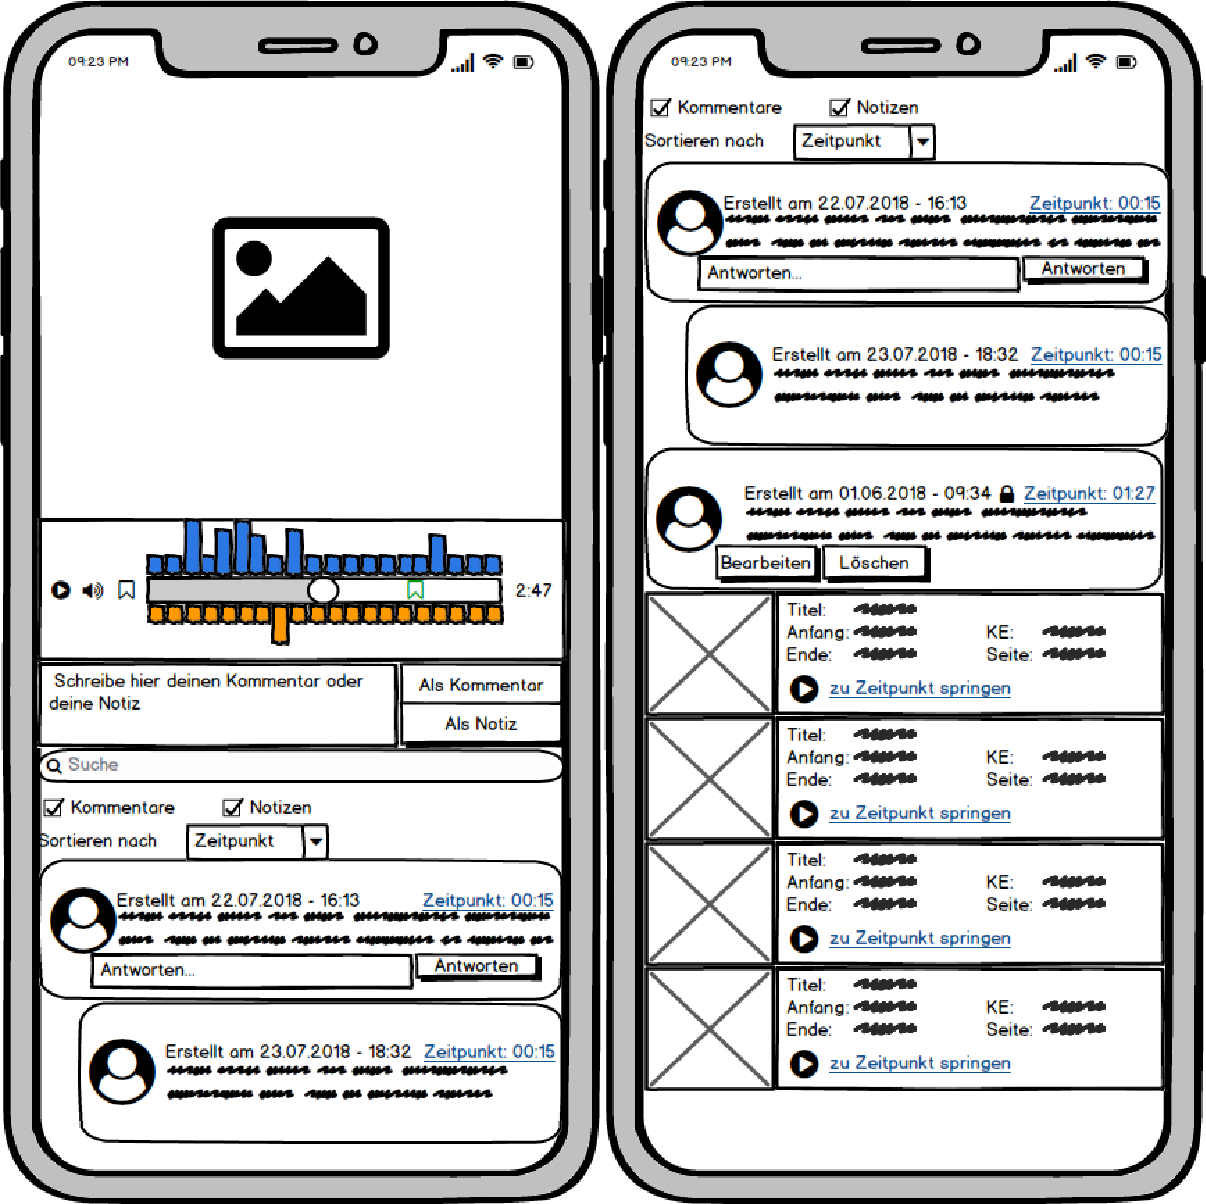
\includegraphics[width=0.8\textwidth,center]{MockupMobile.pdf}
\caption{\label{fig:MockupMobile} Benutzeroberfläche - Mobile Darstellung}
\end{figure}

%%%%%%%%%%
\section{Zusammenfassung}
In diesem Kapitel wurden die grundlegenden konzeptuellen Entscheidungen getroffen. So wurden zu Beginn die Komponenten von Hyperaudio"=Dokumenten im Sinne dieser Arbeit sowie deren Zusammenhänge bestimmt. Daraufhin wurde der Aufbau einer Konfigurationsdatei erarbeitet, welche diese Zusammenhänge abbilden kann. Auch der Datenbankentwurf wurde basierend auf diesen Ergebnissen vorgenommen. Nach dem Abschluss der technischen Konzeption wurde das Design des Plugins entworfen. Anhand verschiedener Mockups wurden Alternativen verglichen und ein Designkonzept beschlossen, das sowohl die Darstellung in Desktop-Umgebungen als auch auf mobilen Endgeräten umfasst.
